\hypertarget{seccion:IniciarSesion}{\vspace{1pt}}
\section{Introduccion}
%\subsection{Administrar pagos admisión}



Para que la ELD pueda mantener actualizado el status de pago de los aspirantes que realizaron la operación en sucursal bancaria, es necesario que el \textbf{Contador General} actualice de forma manual dichos pagos, esto se logra con ayuda del archivo brindado por BANAMEX, el cual servirá para ser cargado en el sistema y este lo interprete y determine si es correcto, en caso de ser correcto actualizar el estado de pago de los aspirantes que allí se encuentran, de lo contrario mostrar las inconsistencias.\\
Una de las operaciones que brinda el sistema, es la actualización manual del status de pago de un aspirante, esta acción le permite tener el control para la actualización del status de pago de los aspirantes, esto con la finalidad de no depender del archivo de BANAMEX en caso de que presentaran conflictos con el mismo.
%\subsubsection{Procedimiento}
\begin{enumerate}
	\item Solicite administrar los pagos admisión seleccionando la opción \textbf{Administración de pagos} del menú \refIU{fig:menuPrincipalCG}{Menú del Contador General} y posteriormente la opción \textbf{Pagos Admisión} del menú \refIU{fig:menuPagosA}{Menú Pagos Admisión}.
	\item Se mostrará la pantalla \refIU{fig:APA}{Administrar Pagos Admisión}.
	\begin{figure}[!htbp]
		\hypertarget{fig:APA}{\hspace{1pt}}
		\begin{center}
			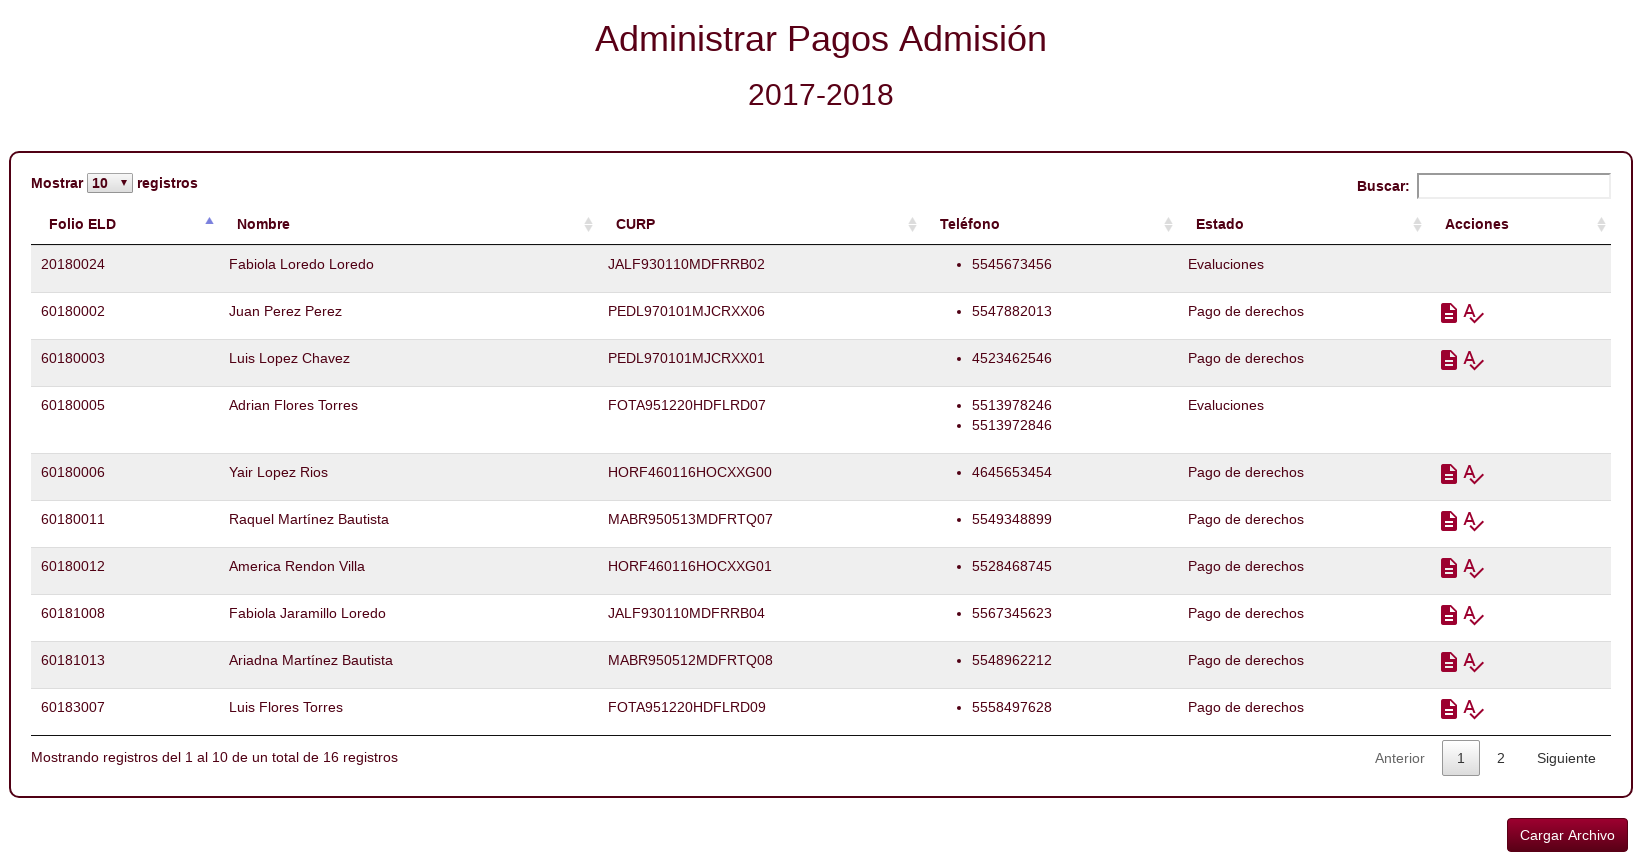
\includegraphics[height=0.3\textheight]{capitulo1/images/IU-APA.png}
			\caption{Administrar Pagos Admisión}
			\label{fig:APA}
		\end{center}
	\end{figure}	
\end{enumerate}
	


\newpage
\begin{Errores}
	\error{El sistema muestra un mensaje indicando que falta información para realizar la operación.}
	{
		\begin{UClist}
			\UCli	Verifique que exista una convocatoria \textbf{Publicada}.
			\UCli	Verifique que exista un periodo de pagos.
			\UCli	Verifique que exista un periodo de pre-registro CENEVAL vigente.
		\end{UClist}
	}
	\error{El sistema muestra un mensaje indicando que no se ha realizado la asociación de fechas de CENEVAL y Psicométrico.}
	{
		\begin{UClist}
			\UCli	Verifique que la Coordinación de Control Escolar haya asociado las fechas CENEVAL y Psicométrico.
		\end{UClist}
	}
	

\end{Errores}
